\chapter{ Fermionic States, its characterisation and the connection with Coding theory.}
Up to this point we provided a detailed explanation of how in quantum mechanical description, reaching equilibrium emerges as a consequence of the structure of quantum mechanics. Even more, we stated that in the case we deal with states which its eigenenergies are close to each other, typicality will also provide us an answer of how this kind of states will reach equilibrium. As we would like to illustrate this phenomena occur, we focus our study in the fermionic case. In this Chapter we are Going to provide a background to understand how fermionic states are usually treated and why we choose to work with them. More specifically, we provide the overview of solvable fermionic systems, its connection to Majorana fermions and Gaussian states, the formalism of Grassmann for anticommuting variables, and the link between all the formalism for fermions and coding theory.\\
\section{Overview}
In many areas of physics one has to has to deal with solving quantum many body problems, which is often a computationally difficult if not impossible task. However, the cases which can be annalitically solved are very well known, and some some assumptions have to be taken into account. In spite of this considerations it has been found that a wide class of complicated Hamiltonians with many-body interactions can be often be mapped onto Hamiltonians that are quadratic in annihilation and creation operators and have the generic form \cite{botero_bcs-like_2004}

\begin{equation}
\hat{H}=\sum_{i j} C_{i j} \hat{a}_{i}^{\dagger} \hat{a}_{j}+\sum_{i j}\left(A_{i j} \hat{a}_{i}^{\dagger}\hat{a}_{j}^{\dagger}+\mathrm{h.c.}\right)
\label{CH2:QuadraticHamiltonian}
\end{equation}

where $i,j$ run from $1$ to the number of modes in the system ($N$) and $\hat{a}_i$, $\hat{a}^{\dagger}_i$ are Fermionic annihilation and creation operators which satisfy the canonical anti-commutation relations (CAR)\cite{fradkin_field_1997}

\begin{equation}
\left\{\hat{a}_{k}, \hat{a}_{l}\right\}=\left\{\hat{a}_{k}^{\dagger}, \hat{a}_{l}^{\dagger}\right\}=0, \quad\left\{\hat{a}_{k}, \hat{a}_{l}^{\dagger}\right\}=\delta_{k l}.
\label{CH2:Anticommutation}
\end{equation}

A convenience when working with these kind of Hamiltonians is that can be diagonalized via a Bogoliubov- Valantin transformations transformation (i.e., canonical transformations), which maps Fermionic creation and annihilation operators on the creation and annihilation operators of non-interacting quasi-particles\cite{berezin_method_1966,bogoljubov_new_1958}. Explicitly the transformation looks like

\begin{equation}
\begin{array}{c}
\hat{a}_{i} \mapsto \gamma_{i} \hat{q}_{i}+\kappa_{i} \hat{q}_{i}^{\dagger}, \\
\hat{a}_{i}^{\dagger} \mapsto \bar{\gamma}_{i} \hat{q}_{i}^{\dagger}+\bar{\kappa}_{i} \hat{q}_{i}.
\end{array}
\label{CH2:Bogoliuvov}
\end{equation}

where $\gamma_i , \kappa_i$ are complex numbers such that preserves the canonical anti-commutation relations given by \eqref{CH2:Anticommutation} for $\hat{q}$, $\hat{q}^{\dagger}$\footnote{This relation can also be expresses as a condition over $\gamma_i , \kappa_i$,
\[ \gamma_i ^2+ \kappa_i^2 = 1,\]
and 
\[\left\{\hat{q}_{k}, \hat{q}_{l}\right\}=\left\{\hat{q}_{k}^{\dagger}, \hat{q}_{l}^{\dagger}\right\}=0, \quad\left\{\hat{q}_{k}, \hat{q}_{l}^{\dagger}\right\}=\delta_{k l}.\]
 }.
\\
Many relevant physics models are diagonalizable via a Bogoliubov-Valantin transformations, some examples are the Hubbard model, BCS theory of superconductivity in the mean field or Hartree-Fock approximation, and certain solvable spin-chain models (After a Jordan-Wigner transformation) \cite{fradkin_field_1997}. As we will later explain, an important feature about the class of Hamiltonians described by \eqref{CH2:QuadraticHamiltonian}, if not the most important for the purpose of this project,  is that not only the ground state (quasi-particle vacuum)  but all eigenstates describing a excitation  in a set of quasi-particles, belong to the class of so-called Fermionic Gaussian states\cite{botero_bcs-like_2004}. What is important about this class of states is that are fully characterized by second order correlations, because all the higher moments factorize. This result is very well known and is known as Wick theorem.
\section{Majorana Fermions}
Majorara fermions are fermions such that they are their own antiparticle. In the frame of condensed matter Majorana Fermions (quasi-particles) can be interpreted as a superposition of a electron state and a hole \cite{leijnse_introduction_2012}.
\\
The formalism of Majorana fermions or Majorana modes of the system (with $N$ modes) can be introduce with the operators
\begin{equation}
\hat{c}_{2j-1}=\hat{a}_{j}^{\dagger}+\hat{a}_{j}, \quad \hat{c}_{2j}=(-i)\left(a_{j}^{\dagger}-a_{j}\right).
\label{CH2:majorana}
\end{equation}
In which case its canonical anti-commutation relations (CAR) take the form
\begin{equation}
\left\{\hat{c}_{k},\hat{c}_{l}\right\}=2 \delta_{k l}.
\label{CH2:CAR_majorana}
\end{equation}

The anti-commutation relations is seen to be a consequence of an $\mathbb{R}^{2N}$ Clifford algebra\footnote{By inspection of \eqref{CH2:CAR_majorana} we see that  any linear transformation of the form $\tilde{\gamma}_{\alpha} = O_{\alpha\beta}\gamma_{\beta}$ where $O\in SO(2N)$, the special orthogonal group in $2N$  dimensions}. Transformation in between Fermionic and Majorana operators is achieved by matrix of the block form
\begin{equation}
\Omega=\left(\begin{array}{cc}
\mathbb{I} & \mathbb{I} \\
i \mathbb{I} & -i \mathbb{I}
\end{array}\right),
\end{equation}

and then the map from Fermionic ($\vec{\hat{a}}^{T} = (\hat{a}_1,\ldots,\hat{a}_1^{\dagger},\ldots)$) and Majorana ($\vec{\hat{c}}^{T} = (\hat{c}_1,\ldots,\hat{c}_1^{\dagger},\ldots)$) operators is written as $\Omega\vec{\hat{a}}=\vec{\hat{c}}$.
\\
By changing from Fermionic operators to Majorana operators is possible, and convenient, to define de Fermionic covariance matrix which as we mentioned before, fully characterise Gaussians states\footnote{In comparison to its boson counterpart the fermion Gaussian states have the property that correlation functions for the creation/annihilation operators are completely determined by the two-point functions according to Wick’s theorem \cite{westwanski_general_1973}, and moreover,  since this property is extensible to correlation function pertaining to a reduced subset of the modes, it follows that any partial (reduced) density matrix obtained from $\rho$ remains Gaussian.}.
\section{Fermionic Covariance matrix }
A system of $N$ fermion modes, described by a set of creation and annihilation operators $\hat{a}^{\dagger}, \hat{a}$  and satisfying the  canonical anti-commutations relations in \eqref{CH2:Anticommutation}, is Gaussian if for such system any state $\rho$ can be written as  \cite{cheong_many-body_2003}

\begin{equation}
\rho=\bigotimes_{k=1}^{N} \tilde{\rho}_{k}, \quad \tilde{\rho}_{k}=\frac{1}{2}\left(1-\lambda_{i}\left[\tilde{a}_{i}^{\dagger}, \tilde{a}_{i}\right]\right),
\label{CH2:rho_gaussiano_no_exp}
\end{equation}

for a certain choice of mode basis $\tilde{a}=u_{i}^{j}\hat{a}_{j} + v_{i}^{j}\hat{a}_{j}^{\dagger}$, and with $|\lambda_i|\leq 1$, where the equality holds for pure states. Equivalently, as mentioned before, Gaussian States are fully characterized by their second moments, so an equivalent form of writing $\rho$ is
\begin{equation}
\rho= \frac{1}{Z}\cdot \exp \left[-\frac{i}{4} \hat{c}^{T} G \hat{c}\right],
\label{CH2:rho_gaussiano_exp}
\end{equation}
with $\hat{c} = (\hat{c}_1,\hat{c}_2,\ldots,\hat{c}_{2N})$, the vector of Majorana operators \eqref{CH2:majorana}, $Z$ a normalization constant and $G$ real anti-symmetric $2N\times 2N$ matrix. 
\\
Since $G$ is a skew-symmetric matrix, it can always be brought to the block diagonal form 
\begin{equation}
O G O^{T}=\bigoplus_{i=1}^{N}\left(\begin{array}{cc}
0 & -\beta_{j} \\
\beta_{j} & 0
\end{array}\right) \quad \text { with } \quad O \in \mathrm{SO}(2 \mathrm{N}),
\label{CH2:MatrixG_Williamson}
\end{equation}
by a special orthogonal matrix $O\in SO(2N)$ where the $\beta_{j}$ are called the Williamson eigenvalues of the matrix $G$. 
From equation \eqref{CH2:rho_gaussiano_exp} it is clear that Gaussian states have an interpretation as thermal (Gibbs) states corresponding to a Hamiltonian of the form
\begin{equation}
\hat{H}=\frac{i}{4} \hat{c}^{T}G\hat{c}= \frac{i}{4} \sum_{k>l}G_{kl}\left[\hat{c}_{k},\hat{c}_{l}\right].
\label{CH2:Hamiltonian_majorana}
\end{equation}

and \eqref{CH2:MatrixG_Williamson} shows that every Gaussian state has a normal mode decomposition in terms of $N$ single mode ``thermal states'' of the form \eqref{CH2:rho_gaussiano_no_exp} ($\sim \text{exp}(-\beta \hat{a}^{\dagger}\hat{a})$)\cite{kraus_pairing_2009}. From this is clear, that the state can be fully determined by the expectation values of quadratic operators $(\hat{a}_i^{(\dagger)}\hat{a}_j^{(\dagger)}$ and  $\hat{a}^{\dagger}_i\hat{a}_j)$. So collecting these expectation values in a real and skew-symmetric covariance matrix $\Gamma$ which is defined via
\begin{equation}
\Gamma_{k l}=\frac{i}{2} \operatorname{tr}\left(\rho\left[c_{k}, c_{l}\right]\right).
\label{CH2:Cov_matrix_elements}
\end{equation}
We will be able to bring this anti-symmetric matrix to its block diagonal form, via a canonical transformation.
\begin{equation}
\tilde{\Gamma} = O \Gamma O^{T}=\bigoplus_{i=1}^{M}\left(\begin{array}{cc}
0 & \lambda_{i} \\
-\lambda_{i} & 0
\end{array}\right),
\label{CH2:Williamson_Cov_fermionic_matrix}
\end{equation}
with $\lambda_i\geq 0$ the Williamson eigenvalues.\\
In terms of the creation/annihilation operators obtained from the transformed $\tilde{c}=O\hat{c}$, the Gaussian state $\rho$ takes the form \eqref{CH2:rho_gaussiano_exp} with $\tilde{\Gamma}$ as its Fermionic covariance matrix. It is easy to see that the relation between $G$ and $\Gamma$ is given by $\lambda_{i} = \tanh{\left(\beta_{i}/2\right)}$, for $i=1,2,\ldots,N$\cite{kraus_pairing_2009}. 
\newline
The equivalence between the special orthogonal group in $2N$ dimensions ($SO(2N)$) and the Fermionic Gaussian states, drives to an interesting  property about states describing multi-particles excitations. If $\ket{\textit{vacuum}}$ is the ground state of some Hamiltonian, with annihilation operators $\hat{a}_{i}$ in a given quasi-particle basis, then $\hat{a}_{i}^{\dagger}\ket{\textit{vacuum}} = \hat{c}_{2i}\ket{\textit{vacuum}}$. Meaning that any multi-particle state of this kind is obtained from some transformation (that preserves the canonical anti-commutation relations) of the ground state $\ket{\textit{vacuum}}$, remains Gaussian. In other words, Gaussian states are preserved under any unitary transformation that preserves anti-commutation relations.
\newline 
The fact that all eigenstates of the Hamiltonian in \eqref{CH2:QuadraticHamiltonian} are Gaussian as well as the extension of this property to a reduced subset of the modes, is quite important since a big part of this work is focused on the study of the Fermionic covariance matrix of the $XY$ model.\\
Up to this point we have talked about some generalities about the quadratic Hamiltonians and how these can be brought to its diagonal form to be analytically solved. However, one may wonder how is this connected to some observables, if the Fermionic covariance matrix has something to do in the observables. The answer to these questions will be boarded in the next section in which we will provide the formalism needed to compute observables over anti-commuting variables as well as the differences we will have between bosons and fermions.
\section{Grassmann Approach}
Fermions are one kind of fundamental particles which can be used to represent quantum information, being one posibility to do quantum computation. From Knill, Laflamme and Milburn\cite{knill_scheme_2001} work, we know that it is possible to provide an universal set of operations for quantum computation by just using passive linear objects. Right after this discovery, Terhal, DiVincenzo\cite{terhal_classical_2002} and knill\cite{knill_fermionic_2001} provided a description of the computational capability for Fermionic linear optics (FLO)\footnote{Whenever we are referring to this term, it basically has in consideration a system consisting of non-interacting electrons in a controllable external potential and a detector that measures projectively occupation numbers of single-electron modes.}. These results show that FLO is not a promising way to do quantum computation, since it can be efficiently simulated by classical means, on the other hand, this provides a very interesting tool to study general properties quantum channels for quantum communication.\\
When working with fermions one could think, weather or not is possible to use the same formalisms than the ones used when working with bosons\footnote{By this we mean that it could be also written in its correspond operators of annihilation and creation $\hat{a}^{\dagger}$,$\hat{a}$\cite{noauthor_density_2007}}, and as expected many features between them are shared. More specifically, in the case of FLO, it shares most of the features with a limited version of photon linear optics, where mostly Gaussian states appears\cite{knill_scheme_2001}\footnote{the main reason for this is that a set of states that can be achieved by FLO operations starting from the Fock vacuum is a set of Fermionic Gaussian states, just as the case of its bosonic counterpart.}.\\
It is worth mentioning that some of the results mentioned in here are quite general and can be used even beyond the scope of our work.




%In Quantum Optics the most common states we work with, are the so-called coherent states,  these states are of great importance since these states turned out to be a proper basis for describing all states of electromagnetic field, are also well known for its intrinsic property that the particle number of such states is indefinite, while the phase is determined exactly\cite{QuantumOptics_wolfgang}, therefore these states can be seen as the counter part of the Fock states\footnote{States that belong to the Fock space have the property that their particle number is well defined but not its phase.}\\When working with fermions one could think if weather or not is possible to use the same formalisms than the ones used when working with bosons\footnote{With its operators of annihilation and creation $\hat{a}^{\dagger}$,$\hat{a}$}\cite{noauthor_density_2007}. The study of Fermionic system is know as Fermionic Linear Optics (FLO). FLO shares many features with a limited version of photon linear optics, where mostly Gaussian states appears\cite{knill_scheme_2001}. The main reason for this is that non-interacting fermion, as well as bosons, are described byin the Lagrangian representation  by Gaussian integrals over anti-commutating (commutating) variables\cite{bravyi_lagrangian_2004}. The states achievable with FLO belong to a closure of a low dimensional Lie group\footnote{Growing only quadratically with the number of modes}. The elements of this Lie group are known as  Gaussian operators \cite{knill_fermionic_2001}, which are the states we mentioned in the latter section and we defined as operators that can be represented as an exponential of another operator which is quadratic in the creation/annihilation operators\footnote{Even though this definition is not valid in cases when the operator does not have full rank, the definition we use here fits for the purpose of this work}.\\




\subsection{Fermionic Linear Optics}
In order provide a more specific description of FLO, we start by defining $N$ abstract Fermionic modes which can be defined by creation $\hat{a}_j$ and annihilation $\hat{a}_j^{\dagger}$, $j=1,\ldots,N$, satisfying \eqref{CH2:Anticommutation}. As mentioned above, any state of the system can be generated from the vacuum state $\ket{\textit{vacuum}}$ of the Fock basis, which we define as
\begin{equation}
\ket{N_1,\ldots,N_{N}} = \left(\hat{a}_{1}^{\dagger}\right)^{N_{1}} \cdots\left(\hat{a}_{n}^{\dagger}\right)^{N_{n}}\left|\textit{vacuum}\right\rangle,
\label{CH2:Fock_Space}
\end{equation}
with $N_i\in \{0,1\}$. We have then that any sequence $\{N_i\}$ can be understood as a Fermionic state which comes from a superposition of the Fock basis.\\
When working with FLO, quadratic Hamiltonians govern the dynamics, in which terms associated with individual energy modes, tunneling and bulk dynamics are included. The structure of these Hamiltonians is what allow us conveniently work with operators which generate the \textit{Clifford} algebra ($\mathcal{C}_{2N}$), described in \eqref{CH2:CAR_majorana}. So we will have that any arbitrary operator $X\in \mathcal{C}_{2N}$ will be written as a polynomial in the operators $\{\hat{c}_a\}$ as
\begin{equation}
X=\alpha \hat{I}+\sum_{p=1}^{2 n} \sum_{1 \leq a_{1}<\cdots<a_{p} \leq 2 n} \alpha_{a_{1}, \ldots, a_{p}} \hat{c}_{a_{1}} \cdots \hat{c}_{a_{p}}
\label{CH2:operators_in_clifford}
\end{equation}

with $\alpha=2^{-n} \operatorname{Tr}(X)$. Particularly for the Hamiltonian operator we have that
\begin{equation}
H=\frac{i}{4} \sum_{a, b=1}^{2 N} H_{a b} \hat{c}_{a} \hat{c}_{b},
\label{CH2:Hamiltonian_in_CLifford}
\end{equation}

with $\{H_{a b}\}$ an anti-symmetric $2N\times 2N$ matrix.\\
We may think that when working with fermions could be the same as working with bosons by changing commutators with anti-commutators and changing to a fine algebra. However, this is not the case, as we will show in the next section observables have to be computed by using the corresponding calculus for fermionic systems.

%However, instead of working with the operator of creation/annihilation we instead work with operators described previously in \eqref{CH2:majorana}, which generate the \textit{Clifford} algebra ($\mathcal{C}_{2N}$) described in \eqref{CH2:CAR_majorana}. Thus Hamiltonians of the form \eqref{CH2:QuadraticHamiltonian} can be brought to the form of \eqref{CH2:Hamiltonian_majorana}. Something to stress is the fact that unitary elements of FLO constitute a group of \textit{canonical transformations} $G_{c}\subset U(2^{N})$\footnote{This can be translated as $V\in G_{c}$ if and only if $V= \exp(i\hat{H})$, with $\hat{H}$ from \eqref{CH2:Hamiltonian_majorana}}, making then see the action of a canonical transformation $V\in G_c$ on the operators $\{\hat{c}_a\}$ as a rotation $R\in SO(2N)$.\\
%When working with FLO we could naively think the formulation should be as if we work with bosons, however, this is not the case, certainly, we can make an analogue formulation as the one on bosons. The first problem we deal is that unitary elements of FLO do not preserve the total number of particles, and we do not have a preferred vacuum state, and neither we have a preferred normal ordering of Fermionic operators. Secondly we often would like to treat both pure and mixed states on equal footing\cite{francesco_conformal_1997}. To address these problems we are going show a brief outline of the anti-commutating variables formalism.


\subsection{Grassmann Calculus}
There are a lot of results from the earlier seventies which describe techniques to study systems with infinite number of fermionic modes modes \cite{soper_construction_1978}, nonetheless, the formalism we are going to present here is a specific case where  a finite number of modes is considered, and consist in a customization of the Lagrangian representation for infinite number of Fermionic modes, presented in \cite{bravyi_classical_2005}. 
Consider $\theta_{1},\ldots,\theta_N$ span a N-dimensional complex linear space $\mathbb{C}^{N}$. From the anti-commutation relation we get that for $\theta_{1},\ldots,\theta_N$,
\begin{equation}
\theta_{a}^{2}=0 \quad \text { and } \quad \theta_{a} \theta_{b}+\theta_{b} \theta_{a}=0,
\label{CH2:Grassmann_anticommutation}
\end{equation}

so it is clear that the most general function we can built over the Grassmann algebra with complex coefficients $\mathcal{G}_{N}$ is  a polynomial of $\theta$'s
\begin{equation}
f(\theta)=\alpha+\sum_{p=1}^{n} \sum_{1 \leq a_{1}<\cdots<a_{p} \leq N} \alpha_{a_{1}, \ldots, a_{p}} \theta_{a_{1}} \cdots \theta_{a_{p}},
\label{CH2:Grassmann_function}
\end{equation}
where the coefficients $\alpha_{*}$ are complex numbers. A polynomial $f(\theta)$ will be called \textit{even} if it involves only even powers of $\theta$, nonetheless something to stress is that even elements constitute the center of the Grassmann algebra.\\
It is possible to differentiate functions of Grassmann variables. A partial derivative over $\theta_{a}$ is a linear operator from $\mathcal{G}_{N}$ to $ \mathcal{G}_{N}$, which is defined by
\begin{equation}
\frac{\partial}{\partial \theta_{a}} 1=0, \quad \frac{\partial}{\partial \theta_{a}} \theta_{b}=\delta_{a b},
\label{CH2:Grassmann_diferential}
\end{equation}
and Liebniz's rule
\begin{equation}
\frac{\partial}{\partial \theta_{a}}\left(\theta_{b} f(\theta)\right)=\delta_{a b} f(\theta)-\theta_{b} \frac{\partial}{\partial \theta_{a}} f(\theta).
\label{CH2:Grassmann_diferential_liebniz}
\end{equation}
The equality \eqref{CH2:Grassmann_diferential_liebniz} implies that 
\begin{equation}
\left\{\frac{\partial}{\partial \theta_{a}}, \frac{\partial}{\partial \theta_{b}}\right\}=0
\label{CH2:Grassmann_partial_derivative_anticommutation}
\end{equation}
Since a derivative $\frac{\partial}{\partial\theta_{a}}f(\theta)$ does not depend upon variable $\theta_{a}$, it is sometimes convenient to think about differentiation as a linear operator mapping $\mathcal{G}_{n}$ into $\mathcal{G}_{n-1}$. Such operator is called integration and is denoted as\cite{bravyi_lagrangian_2004} \footnote{Here we will use a compact notation \[\int \mathrm{D} \theta \equiv \int d \theta_{n} \cdots \int d \theta_{2} \int d \theta_{1},\] and the order is chosen such that \[\int D\theta\ \theta_1\cdots\theta_n = 1\]
}
\begin{equation}
\int d \theta_{a} \equiv \frac{\partial}{\partial \theta_{a}}: \mathcal{G}_{n} \rightarrow \mathcal{G}_{n-1}.
\label{CH2:Grassmann_Integration_relation}
\end{equation}

From equation \eqref{CH2:Grassmann_partial_derivative_anticommutation}  we have that
\begin{equation}
\int \mathrm{D} \theta \frac{\partial}{\partial \theta_{a}} f(\theta)=0,
\end{equation}
this equation combined with \eqref{CH2:Grassmann_diferential_liebniz} give us the anti-commuting version of integration by parts.
\newline
With these properties we show the main equation that will help us calculate what is need for the purpose of this work.
\newline
\textit{For a vectors of Grassmann variables  $\vec{\theta}$, $\vec{\eta}$ and complex anti-symmetric matrix $M$ we have}

\begin{equation}
\int \mathrm{D} \theta \exp \left(\frac{i}{2} \theta^{T} M \theta\right)=i^{n} \operatorname{Pf}(M),
\label{CH2:Grassman_property_1}
\end{equation}
and
\begin{equation}
\int \mathrm{D} \theta \exp \left(\eta^{T} \theta+\frac{i}{2} \theta^{T} M \theta\right)= i^{n} \operatorname{Pf}(M)  \cdot \exp \left(-\frac{i}{2} \eta^{T} M^{-1} \eta\right).
\label{CH2:Grassman_property_2}
\end{equation}
In these formulas $\operatorname{Pf}(N)$ is the Pfaffian of a complex antisymmetric matrix $N$ defined as  anti-symmetrized product $\mathcal{A}(N_{1,2}N_{3,4}\cdots N_{2n-1,2n})$ that is
\begin{equation}
\operatorname{Pf}(N)=\frac{1}{2^{n} n !} \sum_{\sigma \in S_{2 n}} \operatorname{sgn}(\sigma) N_{\sigma_{1}, \sigma_{2}} \cdots N_{\sigma_{2 n-1} \sigma_{2 n}}
\label{CH2:Grassmann_Pfaffian}
\end{equation}
\subsection{Gaussian States}

For this part we are going to introduce in a formal way the states we have been talking about in at the beginning of this chapter. Informally we can say that any Gaussian operator can be represented as an exponent of another operator which is quadratic in creation/annihilation operators. When considering an operator $X\in\mathcal{C}_{2N}$ It is natural to assign a polynomial $\omega(X,\theta)\in \mathcal{G}_{2N}$ of $2N$ Grassmann variables defined by.
%Here we introduce the Grassmann version of the covariance matrix approach showed in \cite{bravyi_lagrangian_2004}. It turns out that the connection between these two approaches is the map assigning the Grassmann variable to each Majorana operator.
%\newline
%Consider $X$ to be a linear operator on the Clifford algebra $\mathcal{C}_{2n}$ that is generated by Majorana operators given in \eqref{CH2:majorana}fulfilling the CAR in \eqref{CH2:CAR_majorana}. One can naturally assign a polynomial in Grassmann variables via

\begin{equation}
\omega\left(\hat{c}_{p} \hat{c}_{q} \cdots \hat{c}_{r}, \theta\right)=\theta_{p} \theta_{q} \cdots \theta_{r}, \quad \omega(\hat{\mathbb{I}}, \theta)=1,
\label{CH2:Gaussian_majorana_map_majorana}
\end{equation}
where this definition comes from the general functions in the Grassmann algebra described in \eqref{CH2:Grassmann_function}.
%\footnote{This definition extends by linearity to an arbitrary $X\in \mathcal{C}_{2n}$. It should be enphasized that $\omega$ is just an isomorphism of linear spaces and it has nothing to do with multiplication in the algebras $\mathcal{C}_{2n}$ and $\mathcal{G}_{2n}$}.
\newline
To illustrate what how this map can be done, consider as an example the projector $\hat{a}_1\hat{a}_1^{\dagger}$, which its action is nothing but to project into a state where the first mode is empy. For this precise case we have that the map to Grassmann variables will look as

%Then we define a state in terms of Gaussianity of its Grassmann representation. A quantum state of $n$ fermionic modes is Gaussian if and only if its operator  $\rho\in\mathcal{C}_{2n}$ has a Gaussian Grassmann representation given by 
\begin{equation}
\omega(\hat{a}_1\hat{a}_1^{\dagger}, \theta)=\frac{1}{2} \left(\mathbb{I}+ i \theta_1\theta_2\right) =\frac{1}{2}  \exp \left(i \theta_1\theta_2\right),
\label{CH2:Gaussian_Grassmann}
\end{equation}
where all exponents were defined by a Taylor series.\\
\newline
For any two operators $X,Y\in \mathcal{C}_{2N}$ one can compute the trace by just using a simple formula,
\begin{equation}
\operatorname{Tr}(X Y)=(-2)^{N} \int D \theta D \mu e^{\theta^{T} \mu} \omega(X, \theta) \omega(Y, \mu),
\label{CH2:Trace_grassmann_operators}
\end{equation}
 which can be directly verified.
It is also easy to see that canonical transformations of an operator $X\in\mathcal{C}_{2N}$ are equivalent to an orthogonal change of basis in the space of the Grassmann variables, this is
\begin{equation}
\omega\left(V X V^{\dagger}, \theta\right)=\omega(X, \eta), \quad \eta_{a}=\sum_{b=1}^{2 n} R_{a b} \theta_{b}.
\label{CH2:Transformations_in_Grassmann_Variables}
\end{equation}
So we will define  a Gaussian states of N Fermionic modes as via its density operator $\rho\in\mathcal{C}_{2N}$. We say that a state is Gaussian in  $\mathcal{C}_{2N}$ \textit{iff} its Grassmann representation is as well Gaussian
\begin{equation}
\omega(\rho, \theta)=\frac{1}{2^{n}} \exp \left(\frac{i}{2} \theta^{T} M \theta\right),
\end{equation}
for some $2N\times 2N$ antisymmetric matrix $M$. The matrix $M$ is defined as 
\begin{equation}
M_{a b}=\frac{i}{2} \operatorname{Tr}\left(\rho\left[\hat{c}_{a}, \hat{c}_{b}\right]\right)=\left\{\begin{aligned}
\operatorname{Tr}\left(\rho i \hat{c}_{a} \hat{c}_{b}\right) & \text { for } a \neq b \\
0 & \text { for } a=b
\end{aligned}\right. ,
\end{equation}
which is nothing but the covariance Fermionic matrix defined in \eqref{CH2:Cov_matrix_elements}, meaning that it can be brought to its Williamson form to get its eigenvalues.\\
\newline
Therefore the connection between the Grassmann formalism for Gaussian states and the Fermionic covariance matrix described at the beginning of the chapter, is easily understood by simply assigning the correspondent covariant matrix to the states we work with. Nonetheless, one could be wondering how is this formalism connect to the error correcting code theory. In the next section we will provide a little historical background of how this theory was done and how one can think states of fermions as binary codes. More specifically we will provide the necessary background to link the theory of correcting errors with Fermionic states which are constrained over a shell of energy in the Hilbert Space.
%\begin{equation}
%\Gamma_{a b}=\frac{i}{2} \operatorname{Tr}\left(\rho\left[\hat{c}_{a}, \hat{c}_{b}\right]\right),
%\label{CH2:Correlation_matrix_Grassmann}
%\end{equation}
%which corresponds to the definition in \eqref{CH2:Cov_matrix_elements}.
%\newline
%To illustrate the results we are going to show as an illustrative example the Grassmann representation of the projector in the first mode.
%\subsection{Example: Computing observable in Grassmann representation of the projector}

%Consider the projector $\hat{a}_1\hat{a}_1^{\dagger}$ projecting into a state ``the first mode is empty'', so in terms of Majorana operators we can write.
%\begin{equation}
%\hat{a}_{1} \hat{a}_{1}^{\dagger}=\frac{1}{2}\left(\hat{I}+i \hat{c}_{1} \hat{c}_{2}\right)
%\label{CH2:example_Grassman_1}
%\end{equation}
 %Its Grassmann representation looks as
 %\begin{equation}
 %\omega\left(\hat{a}_{1} \hat{a}_{1}^{\dagger}, \theta\right)=\frac{1}{2}\left(\hat{\mathbb{I}}+i \theta_{1} \theta_{2}\right)=\frac{1}{2} \exp \left(i \theta_{1} \theta_{2}\right)
 %\label{CH2:example_Grassman_2}
 %\end{equation}

%For any operators $X, Y \in \mathcal{C}_{2 n}$ one can compute a trace using the formula \cite{bravyi_lagrangian_2004}
%\begin{equation}
%\operatorname{Tr}(X Y)=(-2)^{n} \int D \theta D \mu e^{\theta^{T} \mu} \omega(X, \theta) \omega(Y, \mu),
%\label{CH2:example_Grassman_3}
%\end{equation}
%which applied to our case reads
%\begin{equation}
%\operatorname{Tr}\left(\rho \hat{a}_{1} \hat{a}_{1}^{\dagger}\right)=(-2)^{n} \int D \theta D \mu e^{\theta^{T} \mu} \omega\left(\hat{a}_{1} \hat{a}_{1}^{\dagger}, \theta\right) \omega(\rho, \mu)
%\label{CH2:example_Grassman_4}
%\end{equation}

%Now, it is convenient to introduce a $2n\times 2n$ matrix $K$ with only non-zero matrix elements $K_{12}=1$ and $K_{21}=-1$, such that we can write $\omega\left(\hat{a}_{1} \hat{a}_{1}^{\dagger}, \theta\right)=\frac{1}{2} \exp \left(\frac{i}{2} \theta^{T} K \theta\right)$, and therefore

%\begin{equation}
%\begin{aligned}
%\operatorname{Tr}\left(\rho a_{1} a_{1}^{\dagger}\right) &=\frac{(-1)^{n}}{2} \int D \theta \exp \left(\frac{i}{2} \theta^{T} K \theta\right) \int D \mu \exp \left(\theta^{T} \mu+\frac{i}{2} \mu^{T} \Gamma \mu\right)=\\
%&=\frac{(-1)^{n}}{2} \operatorname{Pf}(\Gamma) \int D \theta \exp \left(\frac{i}{2} \theta^{T}\left(K-\Gamma^{-1}\right) \theta\right)=\\
%&=\frac{1}{2} \operatorname{Pf}(\Gamma) \operatorname{Pf}\left(K-\Gamma^{-1}\right).
%\end{aligned}
%\label{CH2:example_Grassman_5}
%\end{equation}

%If $\Gamma$ is a singular matrix the last expression may be regularized taking into account that $\operatorname(Pf)(M)^{2}=det(M)$ for any antisymmetric matrix $M$.  Thus we arrive to
%\begin{equation}
%\left[\operatorname{Tr}\left(\rho \hat{a}_{1} \hat{a}_{1}^{\dagger}\right)\right]^{2}=\frac{1}{4} \operatorname{det}(\Gamma K-\mathbb{I}),
%\label{CH2:example_Grassman_6}
%\end{equation}
%where $\mathbb{I}$ is $2n\times 2n$ unit matrix.\\
%The latter result can be used also to deduce the trace of a product of two states ($\rho_1 \rho_2$), with respective correlation matrix $\Gamma_1$ $\Gamma_2$
%\begin{equation}
%\operatorname{Tr}(\rho_1\rho_2)=\frac{1}{2^{n}}\operatorname{Pf}(\Gamma_1) \operatorname{Pf}\left(\Gamma_2-\Gamma_1^{-1}\right).
%\label{CH2:Product_2_states}
%\end{equation}
%It is known that any real $2N\times 2N$ antisymmetric matrix $M$ can be transformed by the adjoint action of $SO(2N)$ into a block diagonal form 
%of the form
%\begin{equation}
%O \Gamma_i O^{T}=\left[\begin{array}{cc}
%0 & D_i \\
%-D_i & 0
%\end{array}\right],
%\label{CH2:Reduction_rotation_matrix}
%\end{equation}
%where $D_{i}$ is a matrix ($N\times N$) with zero in its entries except for its diagonal. The square of  the equation \eqref{CH2:Product_2_states} can be find easily using the equation \eqref{CH2:example_Grassman_6}

%\begin{align}
%\operatorname{Tr}(\rho_1\rho_2)^{2}&=\frac{1}{2^{2n}}\operatorname{det}\left\{\left[\begin{array}{cc}
%0 & D_1 \\
%-D_1 & 0
%\end{array}\right]\cdot\left[\begin{array}{cc}
%0 & D_2 \\
%-D_2 & 0
%\end{array}\right] - \left[\begin{array}{cc}
%\mathbb{I}_{N\times N} & 0 \\
%0 & \mathbb{I}_{N\times N}
%\end{array}\right]
%\right\}\nonumber\\
%&=\frac{1}{2^{2n}}\operatorname{det}\left[\begin{array}{cc}
%-D_1D_2- \mathbb{I}_{N\times N}& 0 \\
%0 & -D_1D_2-\mathbb{I}_{N\times N}
%\end{array}\right] \nonumber\\
%&=\frac{1}{2^{2n}}\left(\prod_{i=1}^{N}D_{1_i}D_{2_i}+1\right)^{2},
%\label{CH2:Trace_2_cov_matrix}
%\end{align}
%where $D_{j_i}$, $j=1,2$ are the $i$-th diagonal element of the matrix $j$.\\
%The last equation give us then a result we would use later on to compute the trace of the product of two different states for the $XY$ model. As mentioned before the results in this chapter could go beyond the scope of this project, nevertheless, by defining Grassmann variables it is possible to extend the results of this project to other fermion models.\\
%In the next chapter we will use all the concepts to the specific case of the XY model chain, and we will provide a full characterization of this model.

\section{Error correcting Code Theory}
In this section we will provide some concepts and definitions in order to understand how the Coding theory can be linked to Fermionic states.\\
In 1948, Claude Shannon presents his extraordinary work named ``A Mathematical Theory of Communication'' \cite{shannon_mathematical_1948} in which he provided a precise measure of the information content of a random variable in terms of its entropy.  His work is divided in two parts the noiseless coding theorem and the noisy channel theorem. For the purpose of our needs we are going to focus only in the second part of his work, which states that a reliable communication is possible if we use schemes such that its rate is less than the capacity of the channel. Even though he never provided an idea of how this schemes could be found, his work is considered one of the most relevant discovery of the century.\\
\begin{figure}
\centering
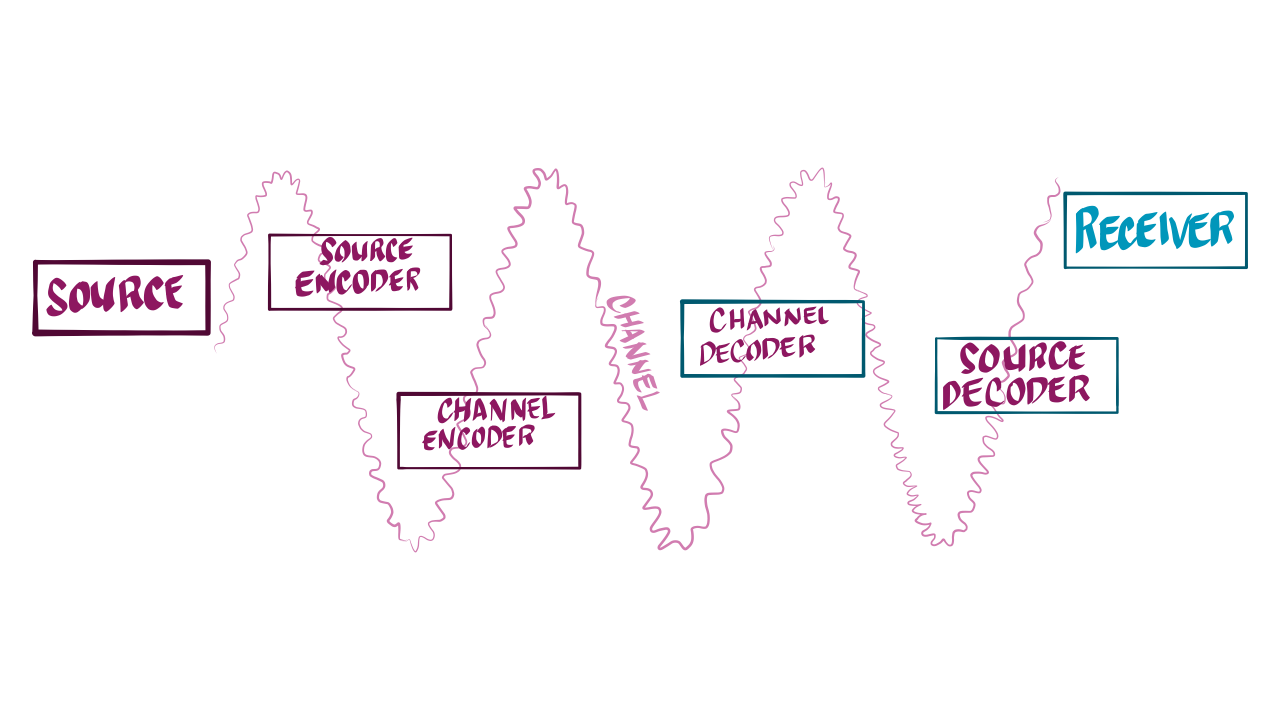
\includegraphics[width=0.9\textwidth]{Figures/Source_Destination.png}
\caption{Representation of the scheme of communication. In the image the noise in the channel is represented by the noise wavy connection between the parts in the communication. }
\label{CH2:Channel_communication}
\end{figure}
\\
Here we will consider codes in communication scenario, as the one showed in figure \ref{CH2:Channel_communication}, meaning that there will be a sender who wants to send $k$ message symbols over a noisy channel and there will be a receiver who has to correct possible errors over the sent code to fully interpret it. The sender will first encodes the $k$ message symbols into $n$ symbols. The receiver then tries to recover the original $k$ message symbols. thus, encoding is the process of adding redundancy and decoding is the process of removing errors and the communication can only be done over the channel. The most fundamental question one can ask is what will be the relation between the amount of redundancy and the errors that can be corrected, and in order to answer this question we will provide some useful definitions.\\

\begin{definition}
  \textbf{Code:}  A code of block $C$ length $n$ over an alphabet $\Sigma$ is a subset of $\Sigma^n$.  If $|\Sigma|=q$, we say that $C$ is a q-ary code.
\end{definition}
it is worth mention that, associated with a code there is also an encoding map $E$ which maps the message set $\mathcal{M}$, identified in some canonical way with $\{1,2,\ldots,|C|\}$ say, to code words belonging to $\Sigma^N$, and thus we have to understand the code as the image of the encoding map.
\begin{definition}
  \textbf{Dimension of a code:}  Given a code $C\subset\Sigma^n$, its dimension is given by
  \begin{equation}
  k \stackrel{\mathrm{def}}{=} \log _{q}|C|,
  \label{CH2:diemnsion_of_code}
  \end{equation}
 \end{definition}
An interesting fact about defining  the dimension of the code in this way is that implicitly it is telling us that when working with codes exponential growth will be always taken into account.\\
We have to provide here a way to measure the amount of redundancy in a given message.
	\begin{definition}
	\textbf{Rate of a code:} The rate of a code with dimension $k$ and block length $n$ is given by 
	\begin{equation}
		R \stackrel{\text { def }}{=} \frac{k}{n},
	\end{equation}
	\end{definition}
this definition is nothing but the average amount of non redundant information each of the $n$ symbols transmitted over the channel.\\ However, an alternative, and more general way of defining this is via the size of the code and the alphabet as
\begin{equation}
R(C)=\frac{\log |C|}{n \log |\Sigma|}.
\end{equation}

\begin{definition}
 \textbf{Hamming distance:} The Hamming distance between two strings $x$ and $y$ of the same length over a finite alphabet $\Sigma$, denoted $\Delta(x,y)$, is defined as the number of positions at which the two strings differ, i.e, $\Delta(x,y) = |\{i| x_i \neq y_i\}|$. The fractional Hamming distance or relative distance between $x,y\in \Sigma^n$ is given by $\delta(x,y) = \frac{\Delta(x,y)}{n}$.
 \end{definition}
It is trivial to check that the Hamming distance defines a metric on $\Sigma^n$.
\begin{definition}
\textbf{Hamming weight:} The Hamming weight of a string $x$ over alphabet $\Sigma$ is defined as the number of non-zero symbols in the string. More formally, the Hamming weight of a string $\mathcal{W}(x) = |\{i| x_i \neq 0\}|$. Note that $\mathcal{W}(x-y) = \Delta(x,y)$.
\end{definition}
Given a string $x\in\Sigma^{N}$, the Hamming ball of radius $r$ around $x$ is the set $\{y\in\Delta^n | \Delta(x,y)\leq r\}$.\\
The minimum distance, or simply distance, of a code $C$, denoted $\Delta(C)$, is defined to be the minimum Hamming distance between two distinct code words of $C$. That is
\begin{definition}
\textbf{Minimum distance:} The minimum distance, or simply distance, of a code $C$, denoted $\Delta(C)$, is defined to be the minimum Hamming distance between two distinct code words of $C$. That is
\begin{equation}
\Delta(C)=\min _{c_{1}, c_{2} \in C \atop c_{1} \neq c_{2}} \Delta\left(c_{1}, c_{2}\right).
\end{equation}
In particular, for every pair of distinct code words in $C$ the Hamming Distance between them is at least $\Delta(C)$
\end{definition}

The relative distance of $C$, denoted $\delta(C)$, is the quantity $\frac{\Delta(C)}{N}$, where $N$ is the block length of $C$. Thus any two code words of $C$ differ in at least a fraction $\Delta(C)$.
\begin{definition}
\textbf{Notation:} A q-ary code of block length $N$ and dimension $k$ will be referred to as an $[N,k]_q$ code. Further, if the code has minimum distance $d$, it will be referred to as an $[N,k,d]_q$ code. When the alphabet size $q$ is clear from the context, or not very relevant to the discussion, we omit the subscript.
\end{definition}

Up to this point we have only described specific codes, codes with fixed block length and dimension. However, since we are interested in the asymptotic behaviour, it turns out to be more useful the study of families of codes instead of an specific code.

\begin{definition}
\textbf{Family of Codes:} Let $q\geq 2$. let $\{n_i\}_{i\geq 1}$ be and increasing sequence of block lengths and suppose there exists sequences $\{k_i\}_{i\geq 1}$ and $\{d_i\}_{i\geq 1}$ such that for all $i\geq 1$ there exist an $[n_i,k_i,d_i]_q$ code $C_i$. then the sequence $C=\{C_i\}_{i\geq1}$ is a family of codes. The rate of C is defined as
\begin{equation}
R(C)=\lim _{i \rightarrow \infty}\left\{\frac{k_{i}}{n_{i}}\right\},
\label{CH2:Rate_of_family_code}
\end{equation}
and the relative distance of $C$ is defined as
\begin{equation}
\delta(C)=\lim _{i \rightarrow \infty}\left\{\frac{d_{i}}{n_{i}}\right\},
\label{CH2:Relative_distance_of_family_code}
\end{equation}
from now on whenever we talk about a code we are implicitly referring to a family of codes.\\
For the purpose of this work, we are going to focus on a particular class of codes, name minimum distance code. This 

\end{definition}







